\section{Random Tree Search Algorithm for Finding NE}\label{sec:apx-alg}
We use random tree search to find the optimum allocation in the CSR game. The search algorithm starts by randomly generating a few allocation as seeds. At each iteration, we pick a sampled allocation (from a buffer) and improve its score by randomly changing a resource of some player in the game.  Over time, we save the best allocations we have seen so far in a buffer. Eventually the algorithm will converge to the optimal allocation in the game.

%n=number of players
%k=number of resources
%q=size of priority-queue


%Random tree setup
Each node in the random tree is $n$-dimensional vector denoting an allocation instance. During simulation, we keep track of the best nodes (allocations) sampled so far, sorted by the score function, in a priority queue of size $q$.

\begin{figure}[htb]
\begin{center}
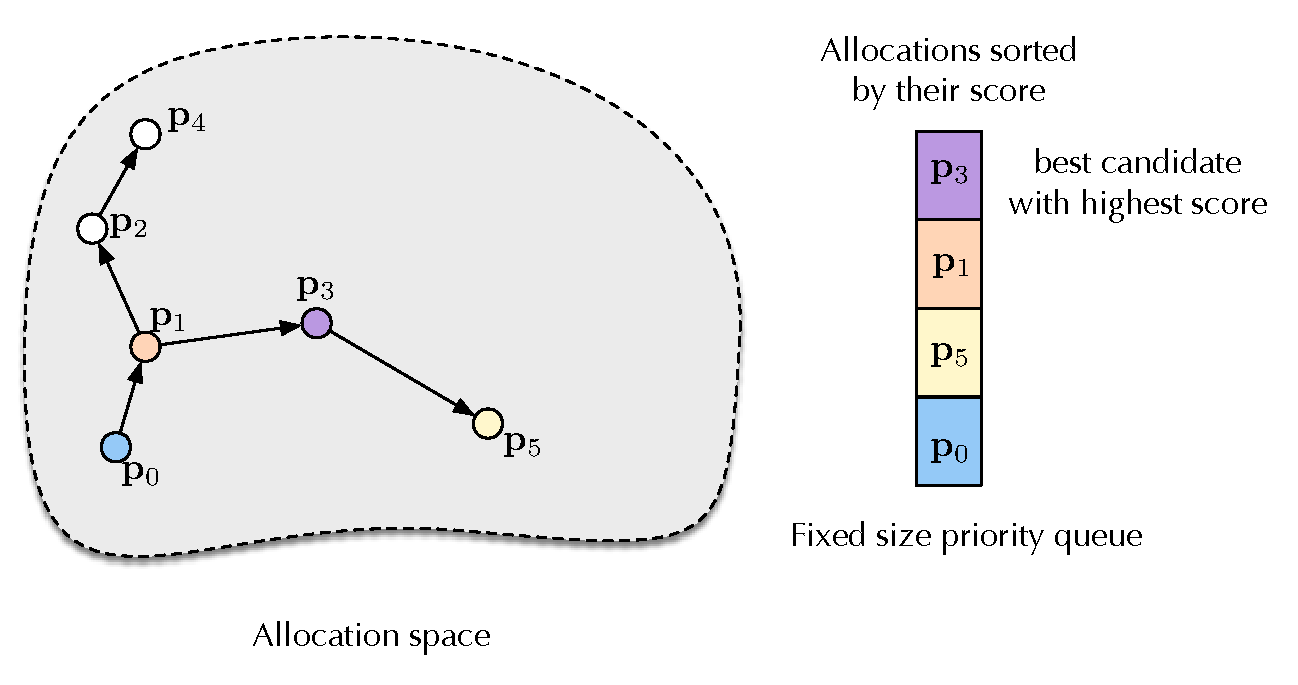
\includegraphics[width=.4\textwidth]{random-tree-figure-1}
\end{center}
\caption{Random tree with 6 sampled allocations ${\bf p}_0\dots {\bf p}_5$. Allocations are sorted in a priority queue of a a fixed size according to their score.}
\label{fig:random_tree_1}
\end{figure}

\begin{figure}[htb]
\begin{center}
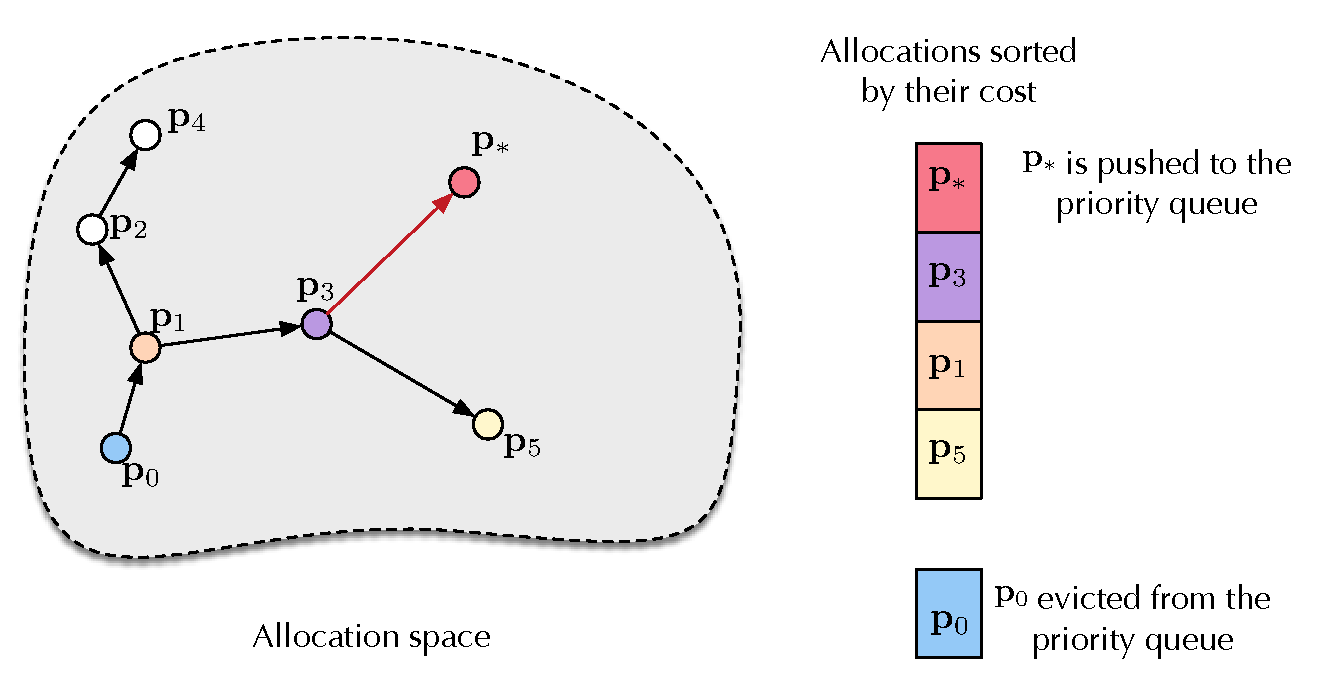
\includegraphics[width=.4\textwidth]{random-tree-figure-2}
\end{center}
\caption{After updating allocation ${\bf p}_3$, we find a new high-scoring allocation ${\bf p}_*$. Pushing ${\bf p}_*$ to the top of the queue evicts the least-scoring allocation ${\bf p}_0$. As a result, we will no longer branch the simulation from ${\bf p}_0$. }
\label{fig:random_tree_2}
\end{figure}

The random tree search algorithm has two phases:
\begin{enumerate}
  \item \emph{Warmup Phase:} Similar to other stochastic search algorithms, the runtime for random tree search depends on the choice of the initial allocation profile. In order to reduce the variance in search, the random tree starts the search by generating multiple randomized allocation as initial states. We emprically observed spending $5\%$ of total samples on finding good initial allocation can substantially reduce overall runtime. The random tree stores the 20 best initial allocation (sorted according to our cost function) and ignores the rest.
  \item \emph{Search Phase:} During the search phase, the random tree picks an allocation from the buffer, changes the resource of one player in the allocation and re-evaluates the radius and number of saturated players in the game. If flipping that node improved the allocation, we insert the new allocation back to the buffer, Otherwise we ignore this step and continue.
\end{enumerate}

The random tree search algorithm work as follows.
Initially, we generate a few random allocation as seends and compute the score of each allocation. Then we push these initial seeds into the fixed-size priority queue sorted by each allocation's score. The froniter set is the set of the $n$ highest scoring allocation that we found so far.
At each iteration, the random tree algorithm pick an allocation from the frontier set, and changes a resource of one of the unsatisfied players. Then the random tree updates the score function and pushes back the new allocation into the frontier set.
If the new allocation has a better score than the lowest-scoring allocation in the frontier set, we drop the least-score element from the frontier set. As a result, the frontier set always has a fixed-size.

\paragraph{Complexity Analysis:}
In order to understand the computational complexity of the random tree search algorithm, we break-down the computation at every iteration. Each iteration in the random tree search consists of three actions:
i) Picking a node from the frontier set (the priority queue) and changing the allocation,
ii) Updating the raidus and saturation of the new allocation, and
iii) Pushing back the new node back to the priority queue.
The computational complexity of the first part is $O(1)$. The most expensive part of the algorithm is updating the radius and saturation of each player, which requires running a breath-first search in the player graph. The computational complexity of running BFS is O(V+E) where $V$ is the number of the players and $E$ is the number of the edges in the CSR graph. Finally, the computational complexity of inserting the new allocation back to the priority queue is $O(log n)$, where $n$ is the size of the fixed priority queue. Finally, we keep the priority queue sorted in order to make weighted sampling, as a result, the complexity of inserting into the priority queue is $O(log(n)\times log(log(n)))$. The overal complexity of the algorithm is $O(V\times(V+E)\times log(n)\times \log\log(n))$.

The random tree search algorithm is probabilistically complete \cite{Lavalle2006}. Therefore, given enought time it will always find the optimal allocation. However, there is no bound on the number of sufficient iterations for finding the optimal allocation. We emprically demonstrate the random tree requires a very few iteration to find the equilibrium points even for very large scale graphs.
